% Pour toute question sur l'utilisation de cette classe, écrivez à jerome.soucy(at)ulaval.ca
% Nécessite la classe Evaluation.sty dans le même dossier ou dans le PATH de votre système
% Nécessite le fichier logo_ul.pdf dans le même dossier un dans le PATH de votre système
\def\Ponderation{25}
\def\SigleNumero{STT-1920}
\def\NomCours{Méthodes statistiques}
\def\DateEvaluation{26 avril 2022 de 10h30 à 12h20}
\def\Session{Été 2021}
\def\NomEvaluation{Examen 3}

% Ne rien mettre entre les accolades si l'enseignant (ou l'enseignante) est aussi le coordonnateur (ou la coordonnatrice)
\def\Coordonnatrice{}
\def\Coordonnateur{}

% Ne rien mettre entre les accolades s'il y a plus d'une section
\def\Enseignant{Julien Miron}
\def\Enseignante{}

% Ne rien mettre entre les accolades s'il s'agit d'un cours à section unique
% Mettre le nom de chacun des enseignants et enseignantes entre les accolades
% Une case à cocher sera générée pour chacune des sections
\def\SectionA{}
\def\SectionB{}
\def\SectionC{}
\def\SectionD{}

% Concerne seulement les travaux pratiques : écrire entre les accolades le nombre maximal de membres pour une équipe
\def\NombreLignes{}		

% Si vous souhaitez q'apparaisse une déclaration d'honneur au bas de la première page, écrivez quelque chose entre les accolades
\def\EnLigne{}

\def\Directives{
\begin{enumerate}
\item Matériel autorisé:
\begin{itemize}
\item Calculatrice scientifique {\bf autorisée par la faculté des sciences et de génie};
\item Une seule feuille aide-m\'emoire \textbf{manuscrite} de format lettre (8.5''$\times$11'') recto-verso.
\end{itemize}
\item Assurez-vous que cette \'evaluation comporte \numquestions ~questions (incluant 1 question bonus) réparties sur \numpages{}~pages, pour un total de \numpoints{}~points et \numbonuspoints{}~points bonus.\
\item \textbf{Veuillez ne pas débrocher votre examen.}
\item Les tables de lois se trouvent à la fin du cahier d'examen aux pages 23 à 28. \textbf{Veuillez ne rien débrocher!}
\item Veuillez déposer votre carte d'identité \textbf{admise} avec photo sur votre bureau.\
\item Vous devez justifier votre raisonnement, sauf pour les questions à choix de réponse et les questions vrai ou faux.\
\item Répondez aux questions sur le questionnaire dans les cases prévues à cet effet. \textbf{Seules les réponses écrites dans les encadrés correspondants seront corrigées.} Il en va de même pour les questions à choix multiples! 
\item Le verso des feuilles peut être utilisé comme brouillon, \textbf{mais ne sera pas corrigé}. Attention à ne rien débrocher.
\end{enumerate}
}

% Veuillez indiquer le type d'évaluation entre crochets
% Examen : option à choisir pour un examen présentiel qui sera corrigé de manière classique. Un tableau des points sera affiché sur la page couverture.
% Gradescope : option à choisir pour un examen qui sera corrigé via Gradescope. Aucun tableau de pointage n'apparaîtra et il y a quelques différences au niveau de la mise en page
% TPS :
% TPF :
% Devoir :
\documentclass[Gradescope]{Evaluation}
\usepackage{multicol,graphicx}
\begin{document}


%%%%%%%%%%%%%%%% QUESTION %%%%%%%%%%%%%%%%
\begin{questions}
\question[3] Soit la table d'ANOVA suivante obtenue à l'aide de \texttt{Rcmdr}:
\begin{verbatim}
>summary(AnovaModel)
            Df   Sum Sq   Mean Sq   F value    Pr(>F)    
Saumons     4    926.12    231.53    238.72    0.0001 
Residuals   48    46.55      0.97                      
\end{verbatim}

À partir de la table d'ANOVA, quelle affirmation parmi les suivantes est vraie?



\begin{itemize}[label = { }]
\item A) La proportion de la variance totale expliquée par le facteur \texttt{Saumons} est égale à $0,0001$. 
\item B) Nous avons 4 niveaux différents pour le facteur \texttt{Saumons}.
\item C) La variance du facteur \texttt{Saumons} est environ 20 fois plus grande que la variance du facteur \texttt{Residuals}.
\item D) L'hypothèse nulle suppose que les moyennes des différents niveaux du facteur \texttt{Saumons} étaient toutes égales.
\end{itemize}

 


\begin{solution}
B)
\end{solution}

%%%%%%%%%%%%%%%% QUESTION %%%%%%%%%%%%%%%%
\question[3] Laquelle des affirmations suivantes est vraie?
\begin{itemize}[label = {}]
\item A) Le modèle d'analyse de la variance à deux facteurs permet de contrôler la variabilité due à un facteur qui ne nous intéresse pas.
\item B) Le modèle d'analyse de la variance à deux facteurs est $Y_{ijk}=\mu+\tau_{i}+\beta_{j}+E_{ijk}$
\item C) Si de l'interaction est présente dans un modèle d'ANOVA à deux facteurs, cela veut dire que l'effet d'un facteur dépend du niveau de l'autre facteur.
\item D) Pour que la conclusion d'une ANOVA à deux facteurs soit valide, au moins un des postulats doit être respecté.
\end{itemize}
 


\begin{solution}
C)
\end{solution}


\newpage
%%%%%%%%%%%%%%%% QUESTION %%%%%%%%%%%%%%%%
\section*{Mise en situation - Questions 3 et 4}
Un ingénieur souhaite comparer la performance de trois marques de freins à disque pour vélo de route. La variable d'intérêt sera donc la distance de freinage parcourue pour passer de 40km/h à 0km/h. L'expérience est répétée $k$ fois pour chaque type de frein. Utilisez la table d'ANOVA suivante pour répondre aux questions 3 et 5.
\begin{verbatim}
            Df    Sum Sq    F value      Pr(>F)    
disque       2     45.77     14.329    0.000001
Residuals   57     91.03      
\end{verbatim}

\question[3] Laquelle des affirmations suivantes est vraie?

\begin{itemize}[label = {}]\setlength{\itemindent}{-2.1em}
\item A) Nous savons que $k=60$.
\item B) L'estimateur de la variance $\sigma^2$ est environ $1,60$.
\item C) La variable réponse est la distance de freinage et le facteur est \texttt{Residuals}.
\item D) Comme il s'agit d'une régression linéaire simple, il n'y a pas de facteur.
\end{itemize}

 

\question[3] Quelle conclusion peut-on tirer à partir de cette table d'ANOVA, au seuil de $1\%$?

\begin{itemize}[label = {}]\setlength{\itemindent}{-2.1em}
\item A) La variance de la distance de freinage d'au moins une marque de frein est différente d'au moins une autre marque.
\item B) La distance de freinage moyenne d'au moins une marque de frein est différente d'au moins une autre marque.
\item C) Comme il y a de l'interaction, nous ne pouvons tirer aucune conclusion sur les facteurs individuels.
\end{itemize}

 


\newpage
\question

Voici quatre sorties obtenues avec \texttt{Rcmdr}.

\smallskip
{\bf Sortie A}
\begin{verbatim}
                  Df     Sum Sq    Mean Sq    F value      Pr(>F)    
FacteurA           3    1049.94     349.98     300.29     0.00001 
FacteurB           2     840.02     420.01     360.38     0.00001 
FacteurA:FacteurB  6    1493.05     248.84     213.51     0.00001 
Residuals         60      69.93       1.17                           
\end{verbatim}

{\bf Sortie B}
\begin{verbatim}
                  Df     Sum Sq.   Mean Sq     F value    Pr(>F)    
FacteurA           3       1.62       0.54      0.4437    0.7226    
FacteurB           2     751.54     375.77    308.4150   0.00001
FacteurA:FacteurB  6       4.26       0.71      0.5825    0.7428    
Residuals         60      73.10       1.22                         
\end{verbatim}


{\bf Sortie C}
\begin{verbatim}
                  Df    Sum Sq    Mean Sq     F value     Pr(>F)    
FacteurA           3    990.23.    330.08    406.3890    0.00001
FacteurB           2    767.49     383.74    472.4639    0.00001
FacteurA:FacteurB  6      4.22       0.70      0.8651     0.5258    
Residuals         60     48.73       0.81               
\end{verbatim}

{\bf Sortie D}
\begin{verbatim}
                  Df     Sum Sq.   Mean Sq    F value    Pr(>F)    
FacteurA           3    148.095     49.365    45.2107   0.00001
FacteurB           2      0.668      0.334     0.3059    0.7376    
FacteurA:FacteurB  6      1.316      0.219     0.2009    0.9752    
Residuals         60     65.513      1.092                        
\end{verbatim}
La page précédente (page 6) contient quatre figures représentant les moyennes des combinaisons de deux facteurs.


Pour chacun des énoncés suivants, inscrivez le \textbf{numéro} de la figure correspondante dans la case.
\begin{parts}
\part[2] La figure qui correspond à la {\bf Sortie A} est la Figure 

\begin{tikzpicture}[baseline=4mm]
\draw (0,0) -- (1,0) -- (1,1) -- (0,1) -- cycle; 
\end{tikzpicture}

\part[2] La figure qui correspond à la {\bf Sortie B} est la Figure 

\begin{tikzpicture}[baseline=4mm]
\draw (0,0) -- (1,0) -- (1,1) -- (0,1) -- cycle; 
\end{tikzpicture}
\part[2] La figure qui correspond à la {\bf Sortie C} est la Figure 
\begin{tikzpicture}[baseline=4mm]
\draw (0,0) -- (1,0) -- (1,1) -- (0,1) -- cycle; 
\end{tikzpicture}
\part[2] La figure qui correspond à la {\bf Sortie D} est la Figure 
\begin{tikzpicture}[baseline=4mm]
\draw (0,0) -- (1,0) -- (1,1) -- (0,1) -- cycle; 
\end{tikzpicture}
\end{parts}
\begin{solution}
\begin{parts}
\part Figure 3
\part Figure 4
\part Figure 2
\part Figure 1
\end{parts}
\end{solution}
\newpage

%%%%%%%%%%%%%%%% QUESTION %%%%%%%%%%%%%%%%

\question

Pour chacune des mises en situation ci-bas, donnez la lettre du modèle qui correspond parmi les suivants: 

\begin{enumerate}[label = \Alph*:]
\item \textbf{Régression linéaire simple}

\item \textbf{Analyse de la variance à un facteur}


\item \textbf{Analyse de la variance à deux facteurs}

\end{enumerate}

\medskip

\begin{parts}
\part[3] Alexis aimerait savoir si le nombre de minutes que ses amis et lui passent à jouer à l'ordinateur à chaque semaine a un impact sur leur note à l'examen final de mathématiques de secondaire 5. Il prévoit donc étudier l'effet des minutes à jouer à l'ordinateur sur la note de l'examen.

 

\part[3] Amandine aimerait comparer la performance de 8 types d'engrais. Elle utilise donc 5 plants de tomates pour chacun des types d'engrais (40 plants au total) et elle mesure la quantité de tomates produites.

 

\part[3] Benjamin veut savoir si le poids des hérissons est impacté par le type de régime de ceux-ci (parmi 3 régimes possibles) ainsi que par le milieu de vie (parmi 2 milieux de vie possibles). Pour chacune des combinaisons de type de régime et de milieu de vie, il soumet 3 hérissons à la combinaison et mesure le poids des hérissons.

 

\part[3] Émile et Léon veulent savoir si la puissance générée par un cycliste a un impact sur le temps d'ascension du fameux \textit{Molard} de Gilly. Ils mesurent donc la puissance moyenne de 25 cyclistes pendant l'ascension ainsi que le temps d'ascension en secondes.

 

\end{parts}







\begin{solution}
\begin{enumerate}
\item B
\item E
\item C
\end{enumerate}
\end{solution}


\newpage



%%%%%%%%%%%%%%%% QUESTION %%%%%%%%%%%%%%%%
\question Déterminez si les énoncés suivants sont vrais ou faux.

\smallskip

\textit{\textbf{Inscrivez «Vrai» ou «Faux» dans les cases appropriées.}}

\begin{parts}
\part[2] Pour que l'analyse de la variance à 1 facteur soit valide, il faut qu'au moins un des postulats soit respecté.

 

\part[2] Lorsqu'un facteur a 2 niveaux, on peut utiliser l'analyse de la variance à un facteur ou un test de Student de comparaison de moyennes avec variances égales pour comparer les moyennes des niveaux.

 

\part[2] En faisant une analyse de la variance à deux facteurs, nous obtenons une \textit{valeur-p} associée à la statistique observée du terme d'interaction égale à $0,001$. Au seuil $\alpha = 0,05$, l'interaction est significative et nous n'interprétons pas les facteurs individuellement.

 

\part[2] Dans un modèle de régression linéaire simple, si l'intervalle de confiance à $95\%$ pour $\beta_0$ est $[0.345; 12.765]$, nous sommes certain qu'une relation linéaire existe entre $X$ et $Y$.

 

\part[2] Dans le contexte d'une régression linéaire simple, nous avons que $y_i=x_i$ pour $i=1, \dots, n$. L'estimateur de $\beta_0$ et l'estimateur de $\beta_1$ valent tous deux~0.

 

\end{parts}

\newpage


%%%%%%%%%%%%%%%% QUESTION %%%%%%%%%%%%%%%%

\question
Une expérience est menée pour étudier l'effet de trois Types d'Essence (A, B et C) et de quatre Types d'Additifs pour essence (W, X, Y et Z) sur la consommation d'essence (en L par 100km) obtenue par un véhicule d'essai. On a évalué aléatoirement $k$ consommations pour chacune des $12$ combinaisons à l'aide d'un plan d'expérience complètement randomisé. On suppose que les postulats sont respectés. Voici une partie d'une sortie Rcmdr. 
\begin{verbatim}
                          Df    Sum Sq    F value        Pr(>F)    
Additifs                  3     52.028    21.1174    0.00004445 
Types.d.essence           2     19.823    12.0690      0.001341 
Additifs:Types.d.essence  6     37.693     7.6496      0.001503 
Residuals                12      9.855                        
\end{verbatim}

\begin{parts}
\part[3] Donnez une estimation de la variance des termes d'erreur, $\sigma^2$. Justifiez votre réponse.

\part[3] Trouvez la valeur de $k$, le nombre de consommations évaluées par combinaison des facteurs. Justifiez.

\part[3] Soit les hypothèses suivantes:
\begin{align*}
& H_0: (\tau\beta)_{ij}= 0\mbox{ pour $i=1,\ldots,a, j=1,\ldots,b$},\\
& H_1: \mbox{ il existe au moins une paire $(i,j)$, pour laquelle $(\tau\beta)_{ij}\neq 0$}. 
\end{align*}
Parmi les décisions suivantes, choisissez celle qui est la bonne au seuil $\alpha=5\%$:
\begin{itemize}[label = {}]
\item A) Nous rejetons $H_0$ au seuil $\alpha = 5\%$.
\item B) Nous ne rejetons pas $H_0$ au seuil $\alpha = 5\%$.
\end{itemize}

 

\part[3] Parmi les conclusions suivantes, choisissez celle qui est la bonne au seuil $\alpha= 5\%$:
\begin{itemize}[label = {}]\setlength{\itemindent}{-3em}
\item A) L'interaction est significative et on peut tester les effets des facteurs individuels à partir de la table d'Anova.
\item B) L'interaction est significative et on ne teste pas les effets des facteurs individuels à partir de la table d'Anova.
\item C) Il n'y a pas d’interaction significative, donc on ne peut rien dire sur les facteurs individuels à partir de la table d'Anova.
\item D) Il n'y a pas d'interaction significative et le facteur Types d'Essence est le seul qui est significatif.
\item E) Il n'y a pas d’interaction significative et le facteur Types d'Additifs est le seul qui est significatif.
\item F) Il n'y a pas d’interaction significative et les deux facteurs sont significatifs.
\end{itemize}
 

\end{parts}
\newpage



%%%%%%%%%%%%%%%% QUESTION %%%%%%%%%%%%%%%%


\question[8]

 Avant de procéder à une ANOVA à un facteur, on veut s'assurer que les conditions d'application du modèle d'analyse de la variance sont respectés. On produit les graphiques ci-dessous pour valider les postulats.
\begin{figure}[!htb]
\centering

\end{figure}

Nommez précisémment deux postulats du modèle que vous devriez vérifier à partir des graphiques ci-haut. Pour chacun d'eux, identifiez les deux figures utiles à sa validation et dites s'il est respecté ou non. Des points seront accordés aux choix de figures et à la conclusion s'ils sont cohérents avec le postulat identifié.

\begin{itemize}[label={$\bullet$}]
    \item \textbf{Postulat:}

\noindent\framebox[17cm]{\rule{0pt}{0.9cm}}  

\medskip

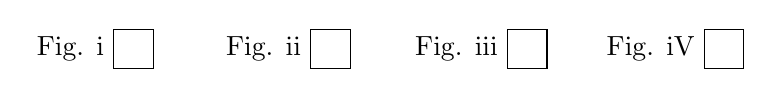
\begin{tikzpicture}    
\draw (0,0) -- (0.5,0) -- (0.5,0.5) -- (0,0.5) -- cycle;    
\draw (0,0.25) node[left]{Fig. i}; 

\draw (2.5,0) -- (3,0) -- (3,0.5) -- (2.5,0.5) -- cycle;    
\draw (2.5,0.25) node[left]{Fig. ii}; 

\draw (5,0) -- (5.5,0) -- (5.5,0.5) -- (5,0.5) -- cycle;    
\draw (5,0.25) node[left]{Fig. iii}; 

\draw (7.5,0) -- (8,0) -- (8,0.5) -- (7.5,0.5) -- cycle;    
\draw (7.5,0.25) node[left]{Fig. iV}; 
\end{tikzpicture}

\textbf{Postulat respecté? }
\medskip

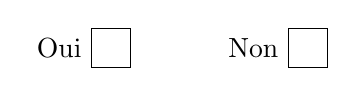
\begin{tikzpicture}    
\draw (0,0) -- (0.5,0) -- (0.5,0.5) -- (0,0.5) -- cycle;    
\draw (0,0.25) node[left]{Oui}; 

\draw (2.5,0) -- (3,0) -- (3,0.5) -- (2.5,0.5) -- cycle;    
\draw (2.5,0.25) node[left]{Non}; 

\end{tikzpicture}

\medskip

\item \textbf{Postulat: }

\noindent\framebox[17cm]{\rule{0pt}{0.9cm}}%  

\medskip

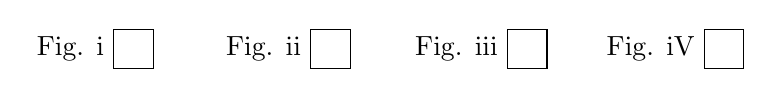
\begin{tikzpicture}    
\draw (0,0) -- (0.5,0) -- (0.5,0.5) -- (0,0.5) -- cycle;    
\draw (0,0.25) node[left]{Fig. i}; 

\draw (2.5,0) -- (3,0) -- (3,0.5) -- (2.5,0.5) -- cycle;    
\draw (2.5,0.25) node[left]{Fig. ii}; 

\draw (5,0) -- (5.5,0) -- (5.5,0.5) -- (5,0.5) -- cycle;    
\draw (5,0.25) node[left]{Fig. iii}; 

\draw (7.5,0) -- (8,0) -- (8,0.5) -- (7.5,0.5) -- cycle;    
\draw (7.5,0.25) node[left]{Fig. iV}; 
\end{tikzpicture}

\textbf{Postulat respecté? }
\medskip 

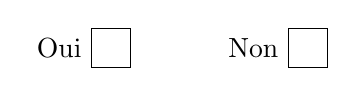
\begin{tikzpicture}    
\draw (0,0) -- (0.5,0) -- (0.5,0.5) -- (0,0.5) -- cycle;    
\draw (0,0.25) node[left]{Oui}; 

\draw (2.5,0) -- (3,0) -- (3,0.5) -- (2.5,0.5) -- cycle;    
\draw (2.5,0.25) node[left]{Non}; 

\end{tikzpicture}
\end{itemize}



\newpage

%%%%%%%%%%%%%%%% QUESTION %%%%%%%%%%%%%%%%
\question\label{rls}
Pour des raisons de santé publique, on s'intéresse à la concentration d'ozone $O_3$ dans l'air (en microgrammes par millilitre). En particulier, on cherche à savoir s'il est possible d'expliquer le taux maximal d'ozone de la journée par la température à midi donnée en degrés celsius. Afin d'étudier le modèle $Y_i=\beta_0+\beta_1 X_i+ E_i$, en supposant que les postulats de régression linéaire sont respectés, vous disposez des résultats suivants:

\begin{verbatim}
Residual standard error: 12.67 on 8 degrees of freedom
Multiple R-squared:  0.7041,	Adjusted R-squared:  0.6671 
F-statistic: 19.03 on 1 and 8 DF,  p-value: 0.002403
\end{verbatim}

\begin{align*}
\sum_{i=1}^{10}x_i=219,1 ; \quad \sum_{i=1}^{10}x_i^2=5214,58;\quad \sum_{i=1}^{10}y_i=1026,4; \quad \sum_{i=1}^{10}y_i^2=118446,6;\quad \sum_{i=1}^{10}x_iy_i=23650,84.
\end{align*}

Vous savez aussi que 

\begin{align*}
    S_{XY} = \sum_{i}^nx_iy_i-n\bar{x}\bar{y}; \quad S_{XX}= \sum_{i}^nx_i^2-n\bar{x}^2.
\end{align*}
\begin{parts}
\part[8] Donnez l'équation de la droite de régression permettant de prédire la concentration d'ozone $O_3$ dans l'air en fonction de la température à midi. Justifiez toutes les étapes de votre démarche.


\part[2] Donnez le pourcentage de la variabilité totale de la concentration d'ozone $O_3$ dans l'air qui est expliquée par la température à midi.


\pagesuivante{\ref{rls}}
\newpage

\suite{\ref{rls}}


\part[3] Calculez la prévision ponctuelle de la concentration d'ozone $O_3$ dans l'air pour une température de $22$ degres.
Justifiez toutes les étapes de votre démarche.


\part[2] Un chercheur aimerait estimer la concentration d'ozone $O_3$ dans l'air en une journée précise. Le midi de cette journée, la température est de $14$ degrés. La prévision ponctuelle de la concentration d'ozone $O_3$ dans l'air en cette journée est environ de $81,83$. Choisissez l'intervalle de valeurs ayant $95\%$ de chances de contenir la concentration d'ozone $O_3$ dans l'air en cette journée. 

\begin{itemize}[label = {}]
\item A) $80,47\pm t_{0,025,n-2}\sqrt{MSE\bigg[\frac{1}{n}+\frac{(14-\bar{x})^2}{S_{XX}}\bigg]}$
\item B) $80,47\pm t_{0,025,n-2}\sqrt{MSE\bigg[1+\frac{1}{n}+\frac{(14-\bar{x})^2}{S_{XX}}\bigg]}$
\end{itemize}
 

\part[1] Si la température à midi ce jour la était de 18 degrés, l'intervalle de valeurs calculé à la question précédente serait...
\begin{itemize}[label = {}]
\item A) plus court
\item B) de même longueur
\item C) plus long
\end{itemize}
 

\part[2] Quelle affirmation parmi les suivantes est vraie au seuil $1\%$?
\begin{itemize}[label = {}]
\item A) La concentration d'ozone $O_3$ dans l'air et la température à midi ne sont pas unis par une relation linéaire significative.
\item B) On ne peut pas prédire la concentration d'ozone $O_3$ dans l'air à partir de la température à midi.
\item C) La concentration d'ozone $O_3$ dans l'air et la température à midi sont indépendantes.
\item D) La relation linéaire entre la concentration d'ozone $O_3$ dans l'air et la température a midi est significative.
\end{itemize}
 

\end{parts}



\newpage
%%%%%%%%%%%%%%%% QUESTION %%%%%%%%%%%%%%%%

\bonusquestion

Supposons un modèle de régression linéaire

\begin{align*}
    Y_i=\beta_0+\beta_1 X_i + \epsilon_i \text{ pour } i = 1,...,n
\end{align*}

où $\epsilon_i \sim \mathcal{U}[-a, a]$, c'est-à-dire une loi uniforme sur [-a, a]. Nous avons les informations suivantes:

 
 \begin{align*}
     E(\epsilon)= 0 & & Var(\epsilon)= \frac{4a^2}{12}
 \end{align*}
 
\begin{parts}
\bonuspart[3] Donnez $E(Y_i)$ et $Var(Y_i)$.
\vspace{3cm}
\bonuspart[3] Quelle est la loi de $Y$? Donnez autant de détails que possible.
\end{parts}

%%%%%%%%%%%%%%%% QUESTION %%%%%%%%%%%%%%%%

\end{questions}
\newpage


\end{document} 
